\documentclass[border=3pt,tikz]{standalone}
% Shared look for every TikZ figure in these notes.
% Included by each standalone figure file; also keeps the figures consistent
% with the colours used in the PDF and on the website.

\usepackage{tikz}
\usepackage{pgfplots}
\pgfplotsset{compat=1.18}
\usetikzlibrary{arrows.meta, decorations.markings, decorations.pathmorphing,
                patterns, calc, positioning}
\usepackage{amsmath}

% Series colours are the three validated categorical slots also used by the
% interactive widgets, so a path drawn in the printed notes and the same path on
% the website are the same colour. They clear the colour-vision-deficiency and
% contrast checks as a set; every path is direct-labelled as well, so colour is
% never the only thing carrying identity.
\definecolor{duPurple}{HTML}{68246D}
\definecolor{duBlue}{HTML}{2A78D6}
\definecolor{duRed}{HTML}{EB6834}
\definecolor{duGreen}{HTML}{1BAF7A}
\definecolor{duGrey}{HTML}{6B6B6B}

\tikzset{
  axisline/.style   = {-{Stealth[length=3mm]}, line width=0.7pt, black},
  path1/.style      = {duBlue,   line width=1.1pt},
  path2/.style      = {duRed,    line width=1.1pt},
  path3/.style      = {duGreen,  line width=1.1pt},
  statedot/.style   = {circle, fill=black, inner sep=1.4pt},
  arrowhead/.style  = {decoration={markings,
                        mark=at position #1 with {\arrow{Stealth[length=2.6mm]}}},
                       postaction={decorate}},
  lbl/.style        = {font=\small},
  slbl/.style       = {font=\footnotesize, duGrey},
  workfill/.style   = {duPurple, opacity=0.16},
}

\begin{document}
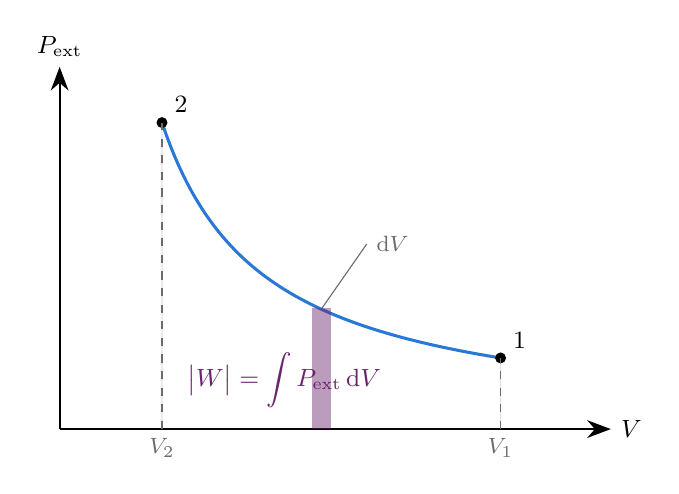
\begin{tikzpicture}[scale=1]
  \def\ya{0.6}
  \draw[axisline] (0,0) -- (7.0,0) node[right, lbl] {$V$};
  \draw[axisline] (0,0) -- (0,4.6) node[above, lbl] {$P_\text{ext}$};

  % the process curve, state 2 (small V, high P) to state 1 (large V, low P)
  \draw[workfill]
    plot[domain=1.3:5.6, samples=80] (\x, {4.6/\x*1.1}) -- (5.6,0) -- (1.3,0) -- cycle;
  \draw[path1] plot[domain=1.3:5.6, samples=80] (\x, {4.6/\x*1.1});

  \node[statedot] at (1.3,{4.6/1.3*1.1}) {};
  \node[statedot] at (5.6,{4.6/5.6*1.1}) {};
  \node[lbl, above right=0pt and 1pt] at (1.3,{4.6/1.3*1.1}) {2};
  \node[lbl, above right=0pt and 1pt] at (5.6,{4.6/5.6*1.1}) {1};

  % the dV strip
  \fill[duPurple, opacity=0.45] (3.2,0) rectangle (3.45,{4.6/3.3*1.1});
  \draw[duGrey, line width=0.4pt] (3.33,{4.6/3.3*1.1}) -- (3.9,2.35);
  \node[slbl, right] at (3.9,2.35) {$\mathrm{d}V$};

  \node[lbl, duPurple, anchor=west] at (1.5,0.62)
    {$\big|W\big| = \displaystyle\int P_\text{ext}\,\mathrm{d}V$};

  \draw[dashed, duGrey, line width=0.4pt] (1.3,0) -- (1.3,{4.6/1.3*1.1});
  \draw[dashed, duGrey, line width=0.4pt] (5.6,0) -- (5.6,{4.6/5.6*1.1});
  \node[slbl, below] at (1.3,0) {$V_2$};
  \node[slbl, below] at (5.6,0) {$V_1$};
\end{tikzpicture}
\end{document}
